\documentclass[11pt]{article}
\usepackage{physics}
\usepackage{graphicx}
\usepackage{tcolorbox}
\usepackage[bb=boondox]{mathalfa}
\usepackage{amsmath}
\usepackage{multicol}
\newcommand\pN{\mathcal{N}}
\usepackage{amssymb}
\usepackage{amsthm}
\newcommand{\Lagr}{L}
\renewcommand{\qedsymbol}{$\blacksquare$}
\makeatletter
\newenvironment{proofw}{\par
	\pushQED{\qed}%
	\normalfont \topsep6\p@\@plus6\p@\relax
	\trivlist
	\item[]\ignorespaces
}{%
	\popQED\endtrivlist\@endpefalse
}
\makeatother

\title{\vspace{-5.0cm}University of Stockholm\\ MT7037-VT19 Statistical Information Theory\\ Final Examination }
\author{Marina Herrera Sarrias }

\begin{document}
\maketitle

\section{Exercise 1}

\begin{tcolorbox}
\textbf{(a)}
Let X and Y be discrete random variables. Show that\\
H ((X+Y)$|$X) = H(Y$|$X). Argue that if X and Y are independent then\\
H(X+Y) $\geq$ H(Y).
\end{tcolorbox}

\begin{proofw}
We wish to prove that the conditional entropy of $Z$ ($Z = g(X,Y) = X + Y$) is the same as the conditional entropy of $Y$ ($Y = Y'$ where $Y' = Z - X$) given $X$. \\

As Z is a function of $(X,Y)$ and the probability of $Z$ taking a value is linked to the probability of $X$ having one. Both probabilities are the same as $Z$ will happen if and only if X happens.

\begin{equation*}
p(Z=z|X=x) = p(Y=z-x|X=x) = p(Y=y'|X=x)
\end{equation*}

We will now prove the equality:\\
\begin{equation} \label{eq1}
\begin{split}
H(Z|X) & = \sum_{} p(x) H(Z|X=x)\\
	   & = \sum_{x \in \chi} p(X= x) \sum_{z \in \mathcal{Z}} p(Z=z|X=x) \log p(Z=z|X=x)\\
	  & = \sum_{x \in \chi} p(X= x) \sum_{y' \in \mathcal{Y'}} p(Y=y'|X=x) \log p(Y=y'|X=x)\\
	   & = \sum_{} p(x) H(Y|X=x)\\
	   & = H(Y|X)\\
\end{split}
\end{equation}

Referring to their entropy we can say that:
\begin{equation*}
 H(X,Y) = H(X) + H(Y|X) \geq  H(g(X,Y)) = H(Z) 
\end{equation*}

and consequently, knowing that conditioning reduces entropy:
\begin{equation*}
H(Z) \geq H(Z|X) = H(Y|X)  
\end{equation*}

In the case that $X$ and $Y$ are independent discrete random variables. We can say that the addition of independent random variables adds uncertainty:

\begin{equation*}
H(Z) \geq H(Z|X) = H(Y|X) = H(Y)
\end{equation*}
or similarly,
\begin{equation*}
H(Z) \geq H(Z|Y) = H(X|Y) = H(X)
\end{equation*}

So, 
\begin{equation*}
\max \{ H(X), H(Y)\} \leq H(Z)
\end{equation*}

%Furthermore, we can also say that:
%\begin{equation*}
%H(X,Y) = H(f(Z), h(Z)) \leq H(Z)
%\end{equation*}
%Finally, in case of independence, the following holds true:
%\begin{equation*}
%H(Z) = H(X) + H(Y)
%\end{equation*}
\end{proofw}
\begin{tcolorbox}
\textbf{(b)}
Show that among all\quad $N$ - valued random variables (i.e. with values
k = 1,2,...) with expected value $\mu$ ,the geometric distributed random variable
with expected value $\mu$ has the maximum value of Shannon entropy.
Reminder: The probability function in a geometric distribution is
$p(k) = {p(1 - p)}^{k-1}, k = 1,2,...$
	
\end{tcolorbox}
\begin{proofw}
Assuming that	
\begin{equation*}
P(X= k) = {p(1 - p)}^{k-1}
\end{equation*}
 Where $k$ and $X$  $\in\mathbb N_{+}$  . Knowing that:
 
\begin{minipage}{.5\linewidth}
	\begin{equation*}
	\sum_{k=1}^{+\infty} (k-1){(1-p)}^{k-1} = \frac{1-p}{{(1-(1-p))}^2}
	\end{equation*}
\end{minipage}
,
\begin{minipage}{.5\linewidth}
	\begin{equation*}
	\sum_{k=1}^{+\infty} {(1-p)}^{k-1} = \frac{1}{(1-(1-p))}\\
	\end{equation*}
\end{minipage}
 \\

The entropy of the geometric distribution is derived as: 
\begin{equation*} \label{}
\begin{split}
H(X) & = - \sum_{k=1}^{+\infty} {p(1-p)}^{k-1} \log p{(1-p)}^{k-1}\\
& = - \sum_{k=1}^{+\infty} {p(1-p)}^{k-1} \log p - \sum_{k=1}^{+\infty}(k-1){p(1-p)}^{k-1} \log (1-p)\\
& = - [\sum_{k=0}^{+\infty} {p(1-p)}^{k} \log p - \sum_{k=0}^{+\infty} k{p(1-p)}^{k} \log {(1-p)}]\\
& = -\frac{p}{1-(1-p)}\log p -\frac{(1-p)}{{(1-(1-p))}^2} \log p(1-p)\\
&= -\log p -\frac{(1-p)}{p} \log p(1-p)\\
\end{split}
\end{equation*}
We are now going to solve the maximization problem:
\begin{equation*} 
\arg \max_{p}\Big(-\sum_{k=1}^{+\infty}p_{k} \log p_{k}\Big)
\end{equation*}
Subject to the constraints: 
\begin{equation*}
\sum_{k=1}^{+\infty} p_{k} = 1
\end{equation*}

\begin{equation*}
\sum_{k=1}^{+\infty}kp_{k} = \mu
\end{equation*}
We will use the Lagrange multipliers to obtain the general form of the $p_{k}$ distribution.
\begin{equation*} 
\begin{split}
\Lagr(p_{k}, \lambda_{1}, \lambda_{2}) & = -\Big(\sum_{k=1}^{+\infty}p_{k} \log p_{k}\Big) + \lambda_{1}\Big(\sum_{k=1}^{+\infty} p_{k}-1\Big) + \lambda_{2}\Big(\sum_{k=0}^{+\infty}kp_{k}-\mu\Big)\\
\end{split}
\end{equation*}

\begin{equation*}
\begin{split}
\pdv{\Lagr}{\lambda_{1}} = 0 &= \sum_{k=1}^{+\infty} p_{k}-1\\
& = {\exp}^{(-1+\lambda_{1})} \sum_{k=1}^{+\infty} {\exp}^{(\lambda_{2})k}\\
&= {\exp}^{(-1 + \lambda_{1})}\Big(\frac{1}{1-{\exp}^{\lambda_{2}}}-1\Big) = 1\\
&= {\exp}^{(-1 + \lambda_{1})}\Big(\frac{{\exp}^{\lambda_{2}}}{1-{\exp}^{\lambda_{2}}}\Big) = 1\\
\pdv{\Lagr}{\lambda_{2}} = 0 &= \sum_{k=0}^{+\infty}kp_{k}-\mu\\
&={\exp}^{(-1+\lambda_{1})}  \sum_{k=1}^{+\infty}k {\exp}^{(\lambda_{2})k}\\
&={\exp}^{(-1+\lambda_{1})}  \frac{{\exp}^{\lambda_{2}}}{{(1-{\exp}^{\lambda_{2}})}^2} = \mu\\
\pdv{\Lagr}{p_{k}} = 0 &= - \log p_{k}-1 + \lambda_{1} +\lambda_{2}k \\
\end{split}
\end{equation*}

Where, 
\begin{equation*}
\begin{split}
\mu &= \frac{1}{1 - {\exp}^{\lambda_{2}}}\\
\lambda_{2} &= \log(\frac{\mu - 1}{\mu})\\
\lambda_{1} &= \log(\frac{1}{\mu-1})+1\\
\end{split}
\end{equation*}
Finally, the $p_{k}$ distribution is derived as:
\begin{equation}\label{lm}
\begin{split}
p_{k} &= {\exp}^{(-1 +\lambda_{1}+\lambda_{2}k)}\\
&= {\exp}^{(-1 +\lambda_{1}+\lambda_{2})}{\exp}^{(k-1)\lambda_{2}}\\
&= \frac{1}{\mu}{\exp}^{(k-1)\lambda_{2}}\\
&= \frac{1}{\mu}{\exp}^{(k-1)\log(\frac{\mu-1}{\mu})}\\
&= \Big(\frac{1}{\mu}\Big)\Big{(\frac{\mu-1}{\mu}\Big)}^{k-1}
\end{split}
\end{equation}

We also know that the mean of the geometric distribution is:
\begin{equation}\label{mean}
\begin{split}
\mu = E[X] &= \sum_{k=1}^{+\infty} k{(1-p)}^{k-1}p\\
&= p \sum_{k=1}^{+\infty} k{(1-p)}^{k-1}\\
&= p \frac{1}{{(1-(1-p))}^{2}}\\
&= \frac{1}{p}
\end{split}
\end{equation}

If we now plug the results obtained in eq.(\ref{mean}) into eq.(\ref{lm}) we can verify that $p_{k}$ is the geometric distribution i.e, the distribution that maximizes the entropy. 

We could also prove it using the Gibb's inequality eq.($\ref{GI}$),  which is just the difference of the Kullback–Leibler divergence eq.($\ref{KL}$). Knowing that the random variable $X$ distributed as $p_{k} \neq 0$ and for the random variable $Y$ distributed as $q_{k}$, where $k \in \mathbb Z^{+}$ 
\begin{equation}\label{KL}
\begin{split}
\mathbb{D}_{KL}(Y|X) &= \sum_{k=1}^{+\infty}q_{k}\log \frac{q_{k}}{p_{k}} \geq 0\\
&= \sum_{k=1}^{+\infty}q_{k}\log q_{k} - \sum_{k=1}^{+\infty}q_{k}\log p_{k}
\end{split}
\end{equation}
\begin{equation}\label{GI}
- \sum_{k=1}^{+\infty}q_{k}\log q_{k} \leq - \sum_{k=1}^{+\infty}q_{k}\log p_{k}
\end{equation}
and knowing that:
\begin{equation*}
H(Y) = - \sum_{k=1}^{+\infty}q_{k}\log q_{k}
\end{equation*}
\begin{equation*}
\begin{split}
- \sum_{k=1}^{+\infty}q_{k}\log p_{k} &= - \sum_{k=1}^{+\infty}q_{k}(\log p + (1-k) \log (1-p))\\
&= - \log p\sum_{k=1}^{+\infty}q_{k} -\sum_{k=1}^{+\infty} q_{k}(1-k) \log (1-p))\\
&= - \log p -\sum_{k=1}^{+\infty} q_{k}(1-k) \log (1-p)\\
&= - \log p -\log (1-p) \sum_{k=1}^{+\infty} q_{k}(1-k)\\
&= - \log p -\log (1-p) \sum_{k=1}^{+\infty} q_{k} + \log (1-p) \sum_{k=1}^{+\infty} k q_{k}\\
&= - \log p -\log (1-p) + \log (1-p) \sum_{k=1}^{+\infty} k q_{k}\\
&= - \log p -\log (1-p) + \log (1-p) \mathbb{E}[Y] \\
&= - \log p +\log (1-p) (\mathbb{E}[Y]-1) \\
&= -\log p -\frac{(1-p)}{p} \log p(1-p) = \mathbb{H}(X)\\
\end{split}
\end{equation*}

\begin{equation*}
\mathbb{H}(Y) \leq \mathbb{H}(X)  
\end{equation*}


\end{proofw}

\begin{tcolorbox}
\textbf{(c)}
Show that\\
$(i)$ H($X_{1}$,$X_{2}$,$X_{3}$) $\leq$ $\frac{1}{2}$ [H($X_{1}$,$X_{2}$) +H($X_{2}$,$X_{3}$) +H($X_{1}$,$X_{3}$)]\\

$(ii)$H($X_{1}$,$X_{2}$,$X_{3}$) $\geq$ $\frac{1}{2}$ [H($X_{1}$,$X_{2}$ $|$$X_{2}$)+H($X_{2}$,$X_{3}$$|$$X_{1}$)+H($X_{1}$,$X_{3}$$|$$X_{2}$)]\\

\end{tcolorbox}
Using the chain rule of entropy we can prove that a collection of random variables are the sum of the conditional entropies, such that:

\begin{equation*}
H(X_{1},X_{2},...,X_{n}) = \sum_{i=1}^{n} H(X_{i}|X_{i-1},...,X_{1})\\
\end{equation*}

We also know that as conditioning reduces entropy:
\begin{equation*}
H(X_{n})\geq H(X_{n}|X_{1}) \geq H(X_{n}|X_{n-1},X_{1})
\end{equation*}
\begin{proofw}
(i)\\

The left hand side of the inequality is:

\begin{equation}\label{LHS}
\begin{split}
H(X_{1},X_{2},X_{3}) & = H(X_{1}) + H(X_{2},X_{3}|X_{1}) \\
& = H(X_{1}) + H(X_{2}|X_{1}) + H(X_{3}|X_{2},X_{1})\\
\end{split}
\end{equation}

While , the right hand side is:
\begin{equation}\label{RHS}
\begin{split}
H(X_{1},X_{2})+H(X_{2},X_{3})+H(X_{1},X_{3}) & = H(X_{1}) + H(X_{2}|X_{1}) + H(X_{2})\\
&= + H(X_{3}|X_{2}) + H(X_{1}) + H(X_{3}|X_{1})\\
&= 2H(X_{1}) + H(X_{2}|X_{1}) + H(X_{2})\\
&= + H(X_{3}|X_{2}) + H(X_{3}|X_{1})
\end{split}
\end{equation}

Now, referring to the results obtained in eq.($\ref{RHS}$) we could also say that:

\begin{equation}\label{proveRHS}
\begin{split}
\frac{1}{2}[H(X_{2})+ H(X_{2}|X_{1})+\\H(X_{3}|X_{2})+H(X_{3}|X_{1})] &\geq  + \frac{1}{2}[H(X_{2}|X_{1})+H(X_{2}|X_{1})+\\ & H(X_{3}|X_{2},X_{1} )+H(X_{3}|X_{2}, X_{1})]\\
&\geq H(X_{2}|X_{1}) + H(X_{3}|X_{2},X_{1} )
\end{split}
\end{equation}

and, because of the above, we can finally prove that:
\begin{equation*}
H(X_{1},X_{2},X_{3}) \leq H(X1) + \frac{1}{2}[H(X_{2})+ H(X_{2}|X_{1})+\\H(X_{3}|X_{2})+H(X_{3}|X_{1})]
\end{equation*}

\end{proofw}

\begin{proofw}
	$(ii)$\\
	
The left hand side of the inequality is the same as in eq.($\ref{LHS}$) while the right hand side is as follows:
\begin{equation}\label{LHSii}
\begin{split}
 &= \frac{1}{2} [H(X_{1},X_{2}|X_{3})+H(X_{2},X_{3}|X_{1})+H(X_{1},X_{3}|X_{2})]\\
& = \frac{1}{2}[H(X_{1}|X_{3})+H(X_{2}|X_{3},X_{1})+H(X_{2}|X_{1})
\\&+H(X_{3}|X_{2},X_{1})+H(X_{1}|X_{2})+H(X_{3}|X_{2},X_{1})]\\
& = H(X_{3}|X_{2},X_{1}) + \frac{1}{2} [H(X_{1}|X_{3})+H(X_{2}|X_{3},X_{1})\\
&+H(X_{2}|X_{1})+H(X_{1}|X_{2})]\\
\end{split}
\end{equation}	

Following the same intuition as in eq.($\ref{proveRHS}$) we can say about the results obtained in eq.($\ref{LHSii}$) that:

\begin{equation*}
\begin{split}
\frac{1}{2} [H(X_{1}|X_{3})+H(X_{2}|X_{3},X_{1})\\+H(X_{2}|X_{1})+H(X_{1}|X_{2})] &\leq \frac{1}{2}[H(X_{2}|X_{1})+H(X_{2}|X_{1}) + H(X_{1}) + H(X_{1})]\\
& \leq H(X_{1}) + H(X_{2}|X_{1})\\
\end{split}
\end{equation*}	

We can now verify that:

\begin{equation*}
\begin{split}
H(X_{1},X_{2},X_{3}) &\geq H(X_{3}|X_{2},X_{1}) + \frac{1}{2} [H(X_{1}|X_{3})+H(X_{2}|X_{3},X_{1}) \\&+H(X_{2}|X_{1})+H(X_{1}|X_{2})]\\
\end{split}
\end{equation*}	
\end{proofw}
\pagebreak
\begin{tcolorbox}
\textbf{(d)}
Suppose that $(X ,Y ,Z)$ are jointly normal distributed and that
$X \rightarrow Y \rightarrow Z \rightarrow$ forms a Markov chain. Let X and Y have the correlation coefficient $\rho1$ and let Y and Z have the correlation coefficient $\rho2$. Find mutual information $I(X;Z)$.
\end{tcolorbox}
\begin{proofw}
The mutual information $I(X;Z)$ is the reduction in the uncertainty of $X$ due to the knowledge of $Z$ and it is represented as:
\begin{equation}\label{eq2}
\begin{split}
I(X;Z) & = H(X) + H(Z) - H(X, Z)\\
       & = H(X) + H(X|Z)\\
\end{split}
\end{equation}

Furthermore the entropy of a normal distribution is derived as:
\begin{equation*}
h(X)  = -\int_{-\infty}^{\infty} \phi(X) \log \phi(X) dx\\
\end{equation*}

Where the density function $\phi(X)$ is:

\begin{equation}\label{eq3}
\phi(X) = \frac{1}{\sqrt{2\pi {\sigma}^2}} \cdot {\exp}^\frac{{-(x-\mu)}^2}{2 {\sigma}^2}\\
\end{equation}

and then, plugging eq.(\ref{eq3}) in eq.(\ref{eq2}) we obtain:

\begin{equation*}
\begin{split}
h(X)  &= -\int_{-\infty}^{\infty} \phi(X) \log (\frac{1}{\sqrt{2\pi {\sigma}^2}} \cdot {e}^\frac{{-(x-\mu)}^2}{2 {\sigma}^2}) dx\\
	  &= -\int_{-\infty}^{\infty} \phi(X) \log \frac{1}{\sqrt{2\pi {\sigma}^2}} dx + \log (e) \int_{-\infty}^{\infty} \phi(X)(\frac{{-(x-\mu)}^2}{2 {\sigma}^2})  dx  \\
	  &= -\int_{-\infty}^{\infty} \phi(X) \log \frac{1}{\sqrt{2\pi {\sigma}^2}} dx - \log (e) \frac{1}{2{\sigma}^2} \int_{-\infty}^{\infty} {(x-\mu)}^2 \phi(X)dx  \\
	  &= \frac{1}{2} \log (2\pi{\sigma}^2) - \log e \frac{1}{2}\\
	  &= \frac{1}{2} [\log 2\pi{\sigma}^2 - \log e]\\
	  &= -\frac{1}{2}\log[ 2\pi e {\sigma}^2]\\	  
\end{split}
\end{equation*}

Since $(X,Y,Z)$ are jointly normal distributed $X$ and $Z$ will also be. Their covariance matrix $\Sigma_{x,z}$ is defined as:
\[
\Sigma_{x,z} =
\begin{bmatrix}
{\sigma_{x}}^2 & \sigma_{x}\sigma_{z}\rho_{xz} \\
\sigma_{x}\sigma_{z}\rho_{xz} & {\sigma_{z}}^2\\
\end{bmatrix}
\]

Now, going back to the mutual information $I(X;Z)$ defined on eq.(\ref{eq2}) we obtain:

\begin{equation*}
\begin{split}
I(X;Z) & = \frac{1}{2}\log(2\pi e {\sigma_{x}}^2) + \frac{1}{2}\log(2\pi e {\sigma_{z}}^2) - \frac{1}{2}\log({2\pi e }^2|\Sigma_{x,z}|)\\
	&= \frac{1}{2}\log(2\pi e {\sigma_{x}}^2) + \frac{1}{2}\log(2\pi e {\sigma_{z}}^2) - \log(2\pi e ) - \frac{1}{2}|\Sigma_{x,z}|\\
\end{split}
\end{equation*}
therefore;
\begin{equation*}
\begin{split}
I(X;Z) & =  - \frac{1}{2}|\Sigma_{x,z}|
\end{split}
\end{equation*}
Where,
\begin{equation*}
\begin{split}
|\Sigma_{x,z}| & = {\sigma_{x}}^2 {\sigma_{z}}^2 - {\sigma_{x}}^2{\sigma_{z}}^2{\rho_{xz}}^2\\
			& = {\sigma_{x}}^2{\sigma_{z}}^2(1-{\rho_{xz}}^2)\\
\end{split}
\end{equation*}

If we now assume that $(X,Y,Z)$ $\sim$ $\pN(0,1)$:

\begin{equation}\label{eq5}
\begin{split}
I(X;Z) & =  -\frac{1}{2}\log	(1 - {\rho_{xz}}^2)\\
\end{split}
\end{equation}

The Markov chain $X \rightarrow Y \rightarrow Z $ implies that the conditional distribution of $Z$ depends only on $Y$ and is conditionally independent of $X$. The joint probability of the random variables $(X, Y, Z)$ is:
\begin{equation*}
p(x,y,z) = p(x)p(y|x)p(z|y)
\end{equation*}
and it implies conditional independence as:
\begin{equation}\label{eq4}
\begin{split}
p(x,z|y) & = \frac{p(x,y,z)}{p(y)}\\
		& = \frac{p(x)p(x|y)p(z|y)}{p(y)}\\
		& = \frac{p(x,y)p(z|y)}{p(y)}\\
		& = \frac{p(x|y)p(y)p(z|y)}{p(y)}\\
		& = p(x|y)p(z|y)
\end{split}
\end{equation}
 
\pagebreak
Then the correlation coefficient $\rho_{xz}$ is obtained as:
\begin{equation*}\label{eq4}
\begin{split}
\rho_{xz} & = \frac{E[XZ]-E[X]E[Z]}{\sigma_{x}\sigma_{z}}\\
		  & =\frac{E[XZ]}{\sigma_{x}\sigma_{z}}\\
		  & =\frac{E[E[XZ|Y]]}{\sigma_{x}\sigma_{z}}\\
		  & =\frac{E [E[X|Y] E[Z|Y]]}{\sigma_{x}\sigma_{z} }\\
		  & =\frac{E[\frac{E[Y]-E[X]cov(X,Y)}{\sigma_{y}} + \frac{cov(X,Y)}{\sigma_{y}}Y][\frac{E[Y]-E[Z]cov(Z,Y)}{\sigma_{y}}+ \frac{cov (Z,Y)}{\sigma_{y}}Y] } {\sigma_{x}\sigma_{z}}\\
		  & =\frac{E[ \frac{cov(X,Y)}{\sigma_{y}}Y][\frac{cov (Z,Y)}{\sigma_{y}}Y]} {\sigma_{x}\sigma_{z}}\\
		  &=\frac{E[\sigma_{x}\rho_{xy}Y][\sigma_{z}\rho_{zy}Y]}{\sigma_{x}\sigma_{z}}\\
		  &=\rho_{xy}\rho_{zy}E[{Y}^{2}]\\
		  &=\rho_{xy}\rho_{zy}
\end{split}
\end{equation*}
Plugging the results into eq.(\ref{eq5}), we can now conclude that:

\begin{equation*}
\begin{split}
I(X;Z) & =  -\frac{1}{2}\log	(1 - {\rho_{xy}}^2{\rho_{zy}}^2)\\
	& =  -\frac{1}{2}\log	(1 - {\rho_{1}}^2{\rho_{2}}^2)\\
\end{split}
\end{equation*}
\end{proofw}
\pagebreak

\section{Exercise 2}
\begin{tcolorbox}
\textbf{(a)}
Define the transfer entropy, starting from Schreiber’s definition in
Phys. Rev. Lett., 85, 461, 2000, in terms of mutual information and Shannon
entropy.
\end{tcolorbox}

The transfer entropy ${T}^{(k,l)}_{\mathbb{Y}\rightarrow \mathbb{X}}(t)$ from the source variable $\mathbb{Y}$ to the target variable $\mathbb{X}$ is the information shared between $\mathbb{Y}$'s past and $\mathbb{X}$'s present given the knowledge of $\mathbb{X}$'s past. it measures how much information the source variable provides about state transitions in the target variable. \\

The random time series processes $\mathbb{X}$ and $\mathbb{Y}$ are a join of sequential processes that evolve over time $t$, with a history length of $k$ for the target variable and $j$ for the source, in which most of the cases $l=1$ or $l=k$ i.e $\mathbb {X}^{(k)}_{t} = (X_{t}, X_{t-1},...,X_{t-k+1})$ and $\mathbb {Y}^{(l)}_{t} = (Y_{t}, Y_{t-1},...,Y_{t-l+1})$.\\

The state of the process $Y$ depends only on its own past and do not depend in any matter on $X$, i.e there is a zero information transfer between $X$ $\rightarrow$ $Y$. Unlike $Y$, the current state of $X$ do not depends on its own past if not it depends probabilistically on the state of $Y$ at the previous time step. i.e $X_{t} = Y_{t-1}$.

\begin{equation*}
\begin{split}
{T}^{(k,l)}_{\mathbb{Y}\rightarrow \mathbb{X}}(t) &= \sum_{X_{t}, {\mathbb{X}_{t-1}}^{(k)},{\mathbb{Y}_{t-1}}^{(l)}} p(x_{t}, {\mathbb{x}_{t-1}}^{(k)},{\mathbb{y}_{t-1}}^{(l)}) \log_{2} \frac{p(x_{t}|{\mathbb{x}_{t-1}}^{(k)},{\mathbb{y}_{t-1}}^{(l)})}{p(x_{t}|{\mathbb{x}_{t-1}}^{(k)})}
\end{split}
\end{equation*}



\begin{equation*}
\begin{split}
 I(X_{t}, {\mathbb{Y}_{t-1}}^{(L)}|{\mathbb{X}_{t-1}}^{(k)}) &= \sum_{X_{t}, {\mathbb{X}_{t-1}}^{(k)},{\mathbb{Y}_{t-1}}^{(l)}} \mathbb{E}_{p({X_{t}, {\mathbb{X}_{t-1}}^{(k)},{\mathbb{Y}_{t-1}}^{(l)}})} \log\frac{p(x_{t}, {\mathbb{y}_{t-1}}^{(l)}|{\mathbb{x}_{t-1}}^{(k)})}{p(x_{t}|{\mathbb{x}_{t-1}}^{(k)}) p({\mathbb{y}_{t-1}}^{(l)}|{\mathbb{x}_{t-1}}^{(k)})}\\
 & = H(X_{t}|{\mathbb{X}_{t-1}}^{(k)}) - H(X_{t}| {\mathbb{Y}_{t-1}}^{(L)}, {\mathbb{X}_{t-1}}^{(k)})
\end{split}
\end{equation*}

\begin{equation*}
\begin{split}
{T}^{(k,l)}_{\mathbb{Y}\rightarrow \mathbb{X}}(t)  = I(X_{t}, {\mathbb{Y}_{t-1}}^{(l)}|{\mathbb{X}_{t-1}}^{(k)}) 
\end{split}
\end{equation*}

${T}^{(k,l)}_{\mathbb{Y}\rightarrow \mathbb{X}}(t)$ measures the deviation from the Markov property which equals the conditional mutual information.
\begin{tcolorbox}
\textbf{(b)}
Why is mutual information not a good measure for an information transfer?
\end{tcolorbox}

\begin{tcolorbox}
\textbf{(c)}
Does Schreiber’s definition of transfer entropy coincide with the
definition of mutual information?
\end{tcolorbox}

\begin{tcolorbox}
\textbf{(d)}
What is the meaning of local transfer entropy?
\end{tcolorbox}

\begin{tcolorbox}
\textbf{(e)}
Is the Granger causality concept the same as transfer entropy?
Explain possible similarities and differences.
\end{tcolorbox}

\begin{tcolorbox}
\textbf{(f)}
To complete this part you need to read the paper by Lizier and Prokopenko in Eur. Phys. J. B 73, 605-615, 2010.
$i)$  Does information transfer have the same meaning as information flow in the opinion of the authors of the paper? Explain possible similarities and differences.\\
$ii)$ What is the difference between interventional and standard
conditional probabilities?
$iii)$ Explain the difference between local transfer entropy and local information flow.\\
$iv)$What are the advantages of the definition of local information flow according to the authors of the paper.\\
\end{tcolorbox}

\section{Exercise 3}

To understand better the concepts of multi-information and its decomposition, this exercise requires you to work out some details in the paper by Schneidman et al., Phys. Rev. Lett., 91, 238701, 2003 discussed in the class.

\begin{tcolorbox}
\textbf{(a)}
For the case of three binary variables (i.e., $x_{1}, x_{2}, x_{3}$ equal to either 0 or1) with all pairwise marginals known, derive with clear steps the maximum entropy distribution in terms of the Lagrange multipliers. Hint: You do not need to solve for the Lagrange multipliers and your answer should look like Eq. 1, namely, the Ising model, in Schneidman et al., Nature, 440, 1007, 2006.
\end{tcolorbox}

\begin{tcolorbox}
\textbf{(b)}
Can you derive $Eq. (8)$ of the paper and correct the typos? Hint: Use the
Venn diagram. This exercise shows that 1) although the area-information
correspondence of the Venn diagram does not hold in the 3-variable case, the Venn
diagram is still useful when deriving relations between different information
quantities; 2) mistakes exist in published papers, so always be critical in reading them.
\end{tcolorbox}

\begin{tcolorbox}
\textbf{(c)}
Show that the connected information of order k in $Eq. (6)$ of the paper
can be written as a relative entropy. When does it equal to zero?
\end{tcolorbox}
\pagebreak

\section{Exercise 4}
\begin{tcolorbox}
\textbf{(a)}
Plot the data points on the x-y plane to see how they look like and
prepare the element-to-element distance matrix $d(\vec{x}_{i},\vec{x}_{j}) = \sqrt{{(x_{i}- x_{j})}^{2}+ {(y_{i}-y_{j})}^{2}}$
$(i,j = 1,2,...,300)$ that will be the input for the clustering algorithm. Also assume each data point carries the same weight, i.e., $p(\vec{x}_{i}) = 1/300$ for all $i$.
\end{tcolorbox}
\begin{figure}[h]
	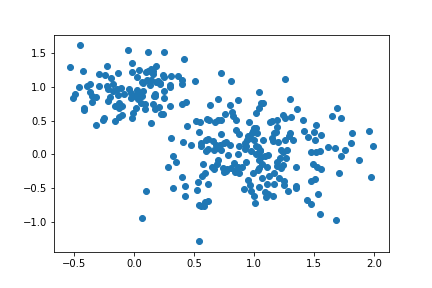
\includegraphics[width=\linewidth]{scatter_plot.png}
\end{figure}

\begin{figure}[h]
	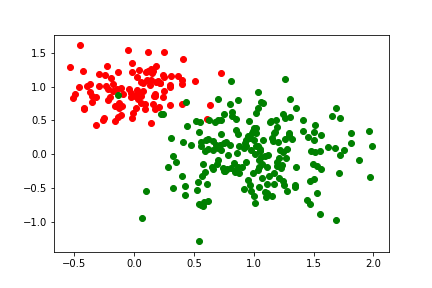
\includegraphics[width=\linewidth]{scatter_plot_clusters_diff.png}
\end{figure}


\pagebreak

\begin{tcolorbox}
\textbf{(b)}
Write a code (no restriction on the program language) to implement
the Blahut-Arimoto algorithm discussed in the class to evaluate the clustering
membership probability,, with fixed number of clusters, and compression distortion tradeoff parameter. Your code should implement a multiple run each
starting with random initial conditions. Note: Your source code should include clear
comments/documentations to describe what is evaluating. We may later randomly ask
a few students, especially those without clear documentations, to demonstrate how
their code works.
\end{tcolorbox}
\pagebreak

\begin{tcolorbox}
\textbf{(c)}
Run your program to construct the information curves for $N_{c}$ = 2, 3 and
4. Hint: choose different values of $\beta$ in between 1 to 50.
\end{tcolorbox}
\pagebreak

\begin{tcolorbox}
\textbf{(d)}
As we have already known that the correct number of clusters is 2,
propose a reasonable way using the quantities evaluated from your code and the information curves to correctly identify the number of clusters. You should clearly explain your rationale and show explicitly which quantities, graphs and/or curves are used in the
identification.
\end{tcolorbox}


\end{document}
